\section{Background: Prior Work and Open Questions}
In what follows, the dataset is denoted by $(x_s,y_s)_{s=1}^n\in\R^{d_{in}}\times \R$ and $y=(y_s,s\in[n])\in\R^n$ denotes the labelling function.

\textbf{Neural Tangent Kernel:}
For a parameter setting $\Theta\in\R^{d_{net}}$, for an input $x\in \R^{d_{in}}$, the \emph{neural tangent feature} (NTF) is given by $\psi_{x,\Theta}=\left(\partial_{\theta}\hat{y}_{\Theta}(x),\theta\in\Theta\right)\in\R^{d_{net}}$. The associated \emph{neural tangent kernel} (NTK) is given by $K_{\Theta}(x,x')=\ip{\psi_{x,\Theta},\psi_{x',\Theta}}$. The NTFs of all the $n$ examples in the dataset can be collected in a NTF matrix $\Psi_{\Theta}=(\psi_{x_s,\Theta},s\in[n])\in\R^{d_{net}\times n}$, and let $K_{\Theta}=\Psi^\top_{\Theta}\Psi_{\Theta}$ be the NTK matrix evaluated on the dataset. Say, we are in the setting, wherein, we are training a over-parameterised DNN using GD procedure to minimise the squared loss $L_{\Theta}=\frac{1}{2}\sum_{s=1}^n \left(\hat{y}_{\Theta}(x_s)-y_s\right)$, Recent works have used the \emph{trajectory based} analysis to show that GD achieves zero training error for this setting. According to the trajectory analysis, the dynamics of the error, $e_t=(\hat{y}_{\Theta_t}(x_s)-y_s,s\in[n])\in\R^n$ can be given by:
\begin{align}
e_{t+1}\approx e_t-\alpha_t K_{\Theta_t} e_t,
\end{align}
where $\alpha_t>0$ is a small step-size used by the GD procedure. Thus, the spectral properties, and in particular, $\rho_{\min}(K_{\Theta_t})$ the minimum eigenvalue of $K_{\Theta_t}$ dictates the rate of convergence.

\textbf{Idealised Regime with Fixed NTK:}
Prior works considered the idealised regime in the limit of infinite width, i.e., width $w\ra\infty$. In this regime, for a DNN of depth $d$, for randomised initialisation, as the width $w\ra\infty$, the following has been shown to hold:\\
$1.$ \cite{arora2019exact} show that the NTK matrix $K_{\Theta_0}\ra K^{(d)}$ as $w\ra\infty$and during training $K_{\Theta_t}$ remains close to $K_{\Theta_0}$ (and hence the NTK can be said to be `fixed' during training). Here $K^{(d)}$ is a deterministic matrix (derived via a recursion similar to the one in \eqref{eq:ntkold}). A trained DNN is equivalent to the kernel regression predictor (with $K^{(d)}$ as the kernel), and hence enjoys the same generalisation ability.\\
$2.$  \cite{cao2019generalization} showed a generalisation bound in the form of $\tilde{\mathcal{O}}\left(d\cdot\sqrt{y^\top K^{(d)} y/n}\right)$\footnote{$a_t=\mathcal{O}(b_t)$ if $\lim\sup_{t\ra\infty}|a_t/b_t|<\infty$, and $\tilde{\mathcal{O}}(\cdot)$ is used to hide logarithmic factors in $\mathcal{O}(\cdot)$.}.\\
\textbf{Expression for $K^{(d)}$} is given by the following recursion: 
\begin{align}\label{eq:ntkold}
&\tilde{K}^{(1)}(s,s')=\Sigma^{(1)}(s,s')=\Sigma(s,s'), M^{(l)}_{ss'}=\left[\begin{matrix}\Sigma^{(l)}(s,s) & \Sigma^{(l)}(s,s')\\ \Sigma^{(l)}(s',s) & \Sigma^{(l)}(s',s')\end{matrix}\right]\in \R^2,\\
&\Sigma^{(l+1)}(s,s')= 2\cdot\mathbb{E}_{(q,q')\sim N(0,M_{ss'}^{(l)})} \left[\chi(q)\chi(q')\right], \dot{\Sigma}^{(l+1)}(s,s')= 2\cdot\mathbb{E}_{(q,q')\sim N(0,M_{ss'}^{(l)})}\left[\dot{\chi}(q)\dot{\chi}(q')\right],\nn\\
&\tilde{K}^{(l+1)}=\tilde{K}^{(l)}\odot \dot{\Sigma}^{(l+1)}+\Sigma^{(l+1)},\nn
\end{align}
where $s,s'\in[n]$ are two input examples in the dataset, $\Sigma$ is the data Gram matrix, $\dot{\chi}$ stands for the derivative of the activation function with respect to the pre-activation input, $N(0,M)$ stands for the mean-zero Gaussian distribution with co-variance matrix $M$. The final limiting matrix is given by $K^{(d)}=\left(\tilde{K}^{(d)}+\Sigma^{(d)}\right)/2$. 

\textbf{Research Gap I (Feature Learning):} In the fixed NTK regime, the DNNs are linear learner using the random NTFs at random initialisation. This implies that there is little or no feature learning. Is this true?\\
\textbf{Research Gap II (Finite vs Infinite):} While pure-kernel methods based on the limiting NTK (i.e., $K^{(d)}$) outperform other state-of-the-art kernel methods, the finite width DNNs (CNNs) still outperform their NTK (CNTK)\footnote{CNTK: Convolutional Neural Tangent Kernel, the NTK for CNNs} counterpart.
\begin{comment}
$1$ A fully-trained wide neural net enjoys the same generalization ability as its corresponding NTK.
$2.$ A fully-trained sufficiently wide ReLU neural network is equivalent to the kernel regression predictor.
$3.$ In the limit, it can be shown that the matrix H(t) remains constant during training i.e., equal to H(0). Moreover, under a random initialization of parameters, the random matrix H (0) converges in probability to a certain deterministic kernel matrix H∗ as the width goes to infinity, which is the Neural Tangent Kernel ker(·,·).
$4.$ 
\end{comment}
\section{Our Contribution}
\textbf{Gate Dynamics and Feature Learning(Resolving Gap I ):}
A major step towards understanding feature learning in DNNs is to tie the \emph{neural path features} to the gates and as a result feature learning to the dynamics of the gates. Three key ingredients that separate this paper from the previous works are i) explicitly allocating separate variable for gating in our analysis, ii) the `path-view', and iii) the `soft-ReLU' gate. We now describe the significance of these three ingredients to the problem of understanding feature learning via gate dynamics.\\
$1.$ The expression for the output $\hat{y}_{\Theta}(x)=\ip{\phi_{x,\Theta},v_{\Theta}}$ reveals that there are two separate learning problems, one that of learning the NPFs and the other that of learning the NPVs. This viewpoint of two learning problems does not naturally emerge in the standard recursive `layer-by-layer' expression for the output of DNNs.\\
$2.$ The gradient (i.e., the \emph{neural tangent feature}) $\psi_{x,\Theta} $naturally splits into two namely the value gradient $\psi^v_{x,\Theta}$ and the feature gradient $\psi^{\phi}_{x,\Theta}$ (see row $5$ of \Cref{tb:compare}) which leads to the following  decomposition (obtained by expanding the expression in  row $6$ of \Cref{tb:compare}) of the NTK matrix:
\begin{align}
K_{\Theta}=K^v_{\Theta}+K^{\phi}_{\Theta}+K^{cross}_{\Theta},
\end{align}
where $K^v_{\Theta}=(\Psi^v_{\Theta})^\top \Psi^v_{\Theta}$ is the Gram matrix of the value gradient, $K^{\phi}_{\Theta}=(\Psi^{\phi}_{\Theta})^\top \Psi^{\phi}_{\Theta}$ is the Gram matrix due to the feature gradient, and $K^{cross}_{\Theta}=(\Psi^v_\Theta)^\top \Psi^{\phi}_{\Theta} +(\Psi^{\phi}_\Theta)^\top \Psi^{v}_{\Theta}$, is a symmetric matrix which is the cross-term obtained as an interaction of the value and the feature gradients.\\
$3.$ The kernel matrices $K^v_{\Theta}$ and $K^{\phi}_{\Theta}$ have different functions, with $K^v_{\Theta}$ captures the dynamics of learning the NPVs keeping for a given NPF and $K^{\phi}_{\Theta}$ capture the dynamics of feature learning.\\
$4.$ The soft-ReLU activation plays a key part: note that, in prior works, in the expression for the limit NTK $K^{(d)}$ in \eqref{eq:ntkold}, $\dot{\chi}$ is either a Heaviside step function or a logit function. Both these functions capture the \emph{on/off} behaviour of the gates, and hence the $K^{(d)}$ captures only the flow of value gradient through the active sub-networks. On the contrary, in the case of soft-ReLU (see row $3$ of \Cref{tb:compare}), $\dot{\chi}_{SR}$ contains both the \emph{on/off} information via the $\dot{\chi}_{SP}$ term as well as the information on the dynamics of sensitive gates via the $\dot{G}_{SR}$ term.
\FloatBarrier
\begin{figure*}[h]\centering
%\begin{minipage}{0.78\columnwidth}
\resizebox{\columnwidth}{!}{
\begin{tabular}{ccc}
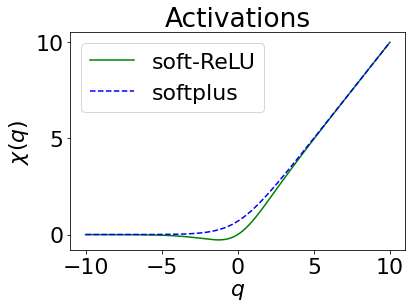
\includegraphics[scale=0.4]{figs/act.png}
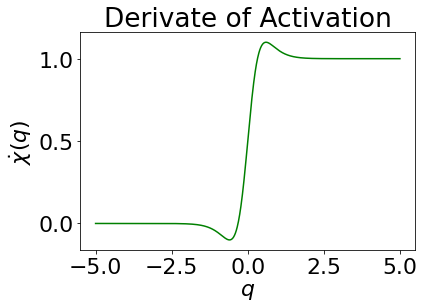
\includegraphics[scale=0.4]{figs/der-act.png}
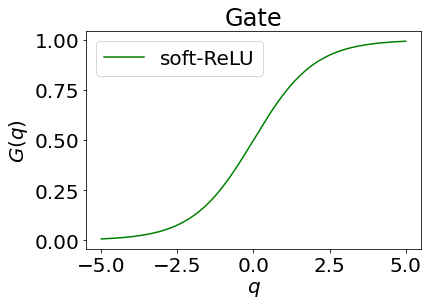
\includegraphics[scale=0.4]{figs/gate.png}
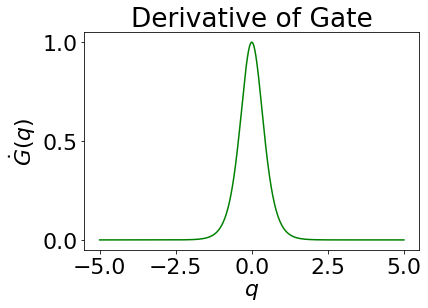
\includegraphics[scale=0.4]{figs/der-gate.png}
%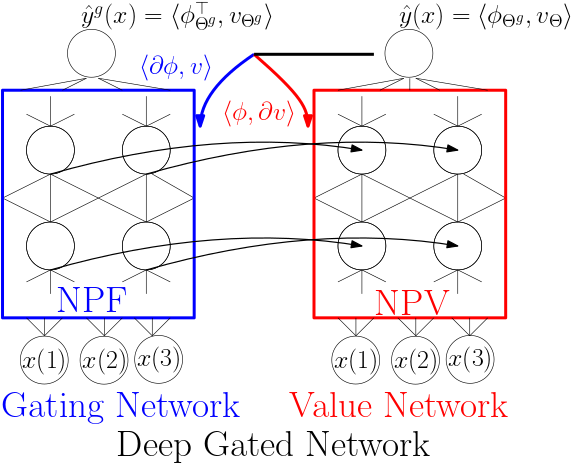
\includegraphics[scale=0.5]{figs/nntwin-blck.png}
%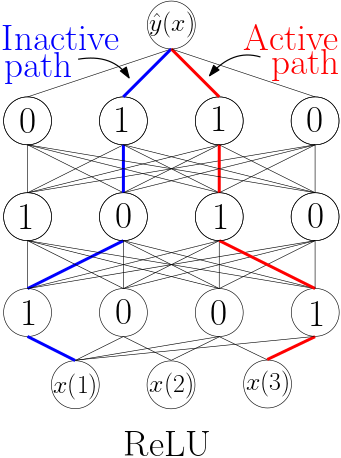
\includegraphics[scale=0.5]{figs/nn.png}
%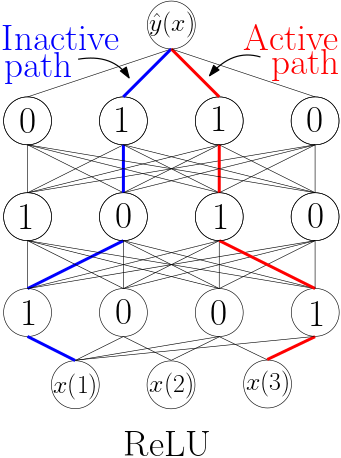
\includegraphics[scale=0.5]{figs/nn.png}
\end{tabular}
}
%\end{minipage}
%\begin{minipage}{0.18\columnwidth}
%\resizebox{\columnwidth}{!}{
%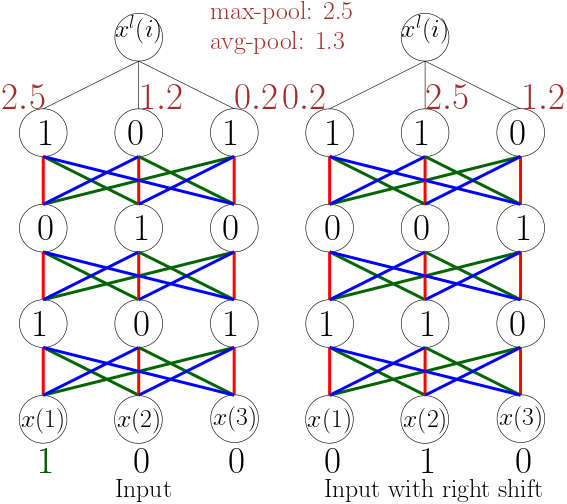
\includegraphics[scale=0.5]{figs/nnconv.png}
%}
%\end{minipage}
\caption{Activations and Gates}
\label{fig:actgate}
\end{figure*}
\begin{table}[h]
\centering
\resizebox{\columnwidth}{!}{
\begin{tabular}{|l|l|l|}\hline
Quantity		&Prior Work																							&Our Work							\\\hline
Gates		&$G_R(q)=\mathbbm{1}_{\{q>0\}}$																			&$G_{SR}(q)=\frac{1}{1+\exp(-\beta q)}$		\\\hline						
Activation		&$\begin{aligned}\chi_{R}(q)&=q\cdot\mathbbm{1}_{\{q>0\}}\\ \chi_{SP}(q)&=\frac{1}{\beta}\log(1+\exp(\beta q))\end{aligned}$			&$\chi_{SR}(q)=q\cdot G_{SR}(q)$					\\\hline				
%$\dot{\chi}$	&$\begin{aligned}\dot{\chi_{R}}(q)&: \text{Heaviside step function} \\ \dot{\chi}_{SP}(q)&=\frac{1}{1+\exp(-\beta q)}\end{aligned}$		&$\dot{\chi}_{SR}(q)=\dot{\chi}_{SP}(q)+\underbrace{\frac{\beta q}{(1+\exp(\beta q))(1+\exp(-\beta q))}}_{\text{Gate Dynamics}}$ \\\hline
$\dot{\chi}$	&$\begin{aligned}\dot{\chi_{R}}(q)&: \text{Heaviside step function} \\ \dot{\chi}_{SP}(q)&=\frac{1}{1+\exp(-\beta q)}\end{aligned}$		&$\dot{\chi}_{SR}(q)=\dot{\chi}_{SP}(q)+\underbrace{\dot{G}_{SR}(q)}_{\text{Gate Dynamics}}$ \\\hline
Output		&$\hat{y}_{\Theta}(x)$: recursive, nested, layer-by-layer 																						&$\hat{y}_{\Theta}(x)=\ip{\phi_{x,\Theta},v_{\Theta}}$\\\hline
%NPF, NPK		&Not Applicable																										&\shortstack[l]{NPF: $\phi_{x,\Theta}$ (see \eqref{eq:npfdef})\\ NPK: $H_{\Theta}(x,x')=\ip{\phi_{x,\Theta},\phi_{x',\Theta}}$}\\\hline
NTF			&$\psi_{x,\Theta}=\left(\partial_{\theta}\hat{y}_{\Theta}(x),\theta\in\Theta\right)\in\R^{d_{net}}$								
&$\begin{aligned}\psi_{x,\Theta}&=\psi^v_{x,\Theta}+\psi^{\phi}_{x,\Theta}\\\psi^v_{x,\Theta}&=\left(\ip{\phi_{x,\Theta}, \partial_{\theta} v_{\Theta}},\theta\in\Theta\right)\in\R^{d_{net}} \\ \psi^{\phi}_{x,\Theta}&=\left(\ip{\partial_{\theta}\phi_{x,\Theta}, v_{\Theta}},\theta\in\Theta\right)\in\R^{d_{net}}\end{aligned}$ \\\hline	
NTK			&$K_{\Theta}(x,x')=\ip{\psi_{x,\Theta},\psi_{x',\Theta}}$														&$K_{\Theta}(x,x')=\ip{\psi^v_{x,\Theta}+\psi^{\phi}_{x,\Theta},\psi^v_{x',\Theta}+\psi^{\phi}_{x',\Theta}}$	\\\hline		
$\dot{\Sigma}^{(l+1)}(s,s')$	&$\dot{\chi}_{SP}(q)\dot{\chi}_{SP}(q')$ &$\begin{aligned}\dot{\chi}_{SP}(q)\dot{\chi}_{SP}(q')&+qq'\dot{G}_{SR}(q)\dot{G}_{SR}(q')\\ +q\dot{G}_{SR}(q)\dot{\chi}_{SP}(q')&+q'\dot{G}_{SR}(q')\dot{\chi}_{SP}(q)\end{aligned}$\\\hline
%$\begin{aligned}\text{Learning}\\\text{Regime}\end{aligned}$			&$\begin{aligned}\text{Fixed NTF:}\quad\quad\quad\quad\quad \\ \hat{y}_{\Theta_0+\Delta \Theta}(x)=\hat{y}_{\Theta_0}(x)+\ip{\psi_{x,\Theta_0}, \Delta\Theta}\end{aligned}$								&$\hat{y}_{\Theta_0+\Delta \Theta}(x)=\hat{y}_{\Theta_0}(x)+\ip{\psi^v_{x,\Theta_0}, \Delta\Theta}$\\\hline
%\shortstack[l]{Idealised\\Regime\\ \quad}			&\shortstack[l]{{Fixed NTF/NTK (for large $w$):} \\ $\hat{y}_{\Theta_0+\Delta \Theta}(x)\approx\hat{y}_{\Theta_0}(x)+\ip{\psi_{x,\Theta_0}, \Delta\Theta}$\\ \quad\\ \quad \\ \quad\\ \quad}								&\shortstack[l]{\quad\\{Fixed NPF/NPK (for large $w$):}\\ $\hat{y}_{\Theta_0+\Delta \Theta}(x)\approx\hat{y}_{\Theta_0}(x)+\ip{\psi^v_{x,\Theta_0}, \Delta\Theta}$ \\ \Cref{sec:optimisation}-\Cref{th:main}}\\\hline


\end{tabular}
}
\caption{A comparison of prior work and our paper. Here subscripts $R$, $SR$ and $SP$ stand for ReLU, soft-ReLU and softplus respectively.}
\label{tb:compare}
\end{table}
$5.$ Plugging the soft-ReLU instead of softplus/ReLU in \eqref{eq:ntkold} will indeed bring in the additional terms related to gate dynamics (see last row of \Cref{tb:compare}) in $K^{(d)}$. However, note that $K^{(d)}$ is a single matrix, and only due to the `path-view', we can identify its components namely $K^v_{\Theta}$, and $K^{\phi}_{\Theta}$ which have completely different functions.
\FloatBarrier
\begin{table}[h]\centering
\resizebox{\columnwidth}{!}{
\begin{tabular}{| l | l | l |}\hline
Standard (finite $w$) &Fixed NTK ($w\ra\infty$) & Fixed NPK (finite $w$)\\\hline
$\dot{\Theta}_t=-\sum_{s=1}^n \psi_{x,t}e_t(s)$ &$\dot{\Theta}_t\approx0$ &$\dot{\Theta}_t=-\sum_{s=1}^n \psi^v_{x,t}e_t(s)$ \\\hline
$\dot{\phi}_{x_s,t}(p)=x(\I_0(p))\sum_{\theta\in\Theta}\partial_{\theta}A_t(x_s,p)\dot{\theta}_t$ &$\dot{\phi}_{x_s,t}(p)\approx 0$ &$\dot{\phi}_{x_s,t}(p)=0$\\\hline
$\dot{v}_t(p)=\sum_{\theta\in\Theta}\partial_{\theta}v_t(p)\dot{\theta}_t$ &$\dot{v}_t(p)\approx 0$ &$\dot{v}_t(p)=\sum_{\theta\in\Theta}\partial_{\theta}v_t(p)\dot{\theta}_t$\\\hline
$\dot{e}_t=-(K^v_t+K^{\phi}_t+K^{cross}_{\Theta})e_t$ &$\dot{e}_t=-K^{(d)}e_t$ &$\dot{e}_t=-K^v_te_t$\\\hline
\end{tabular}
}
\caption{Dynamics in various regimes. Here $p\in[P], s\in[n]$.}
\label{tb:dynamics}
\end{table}
\begin{comment}
\FloatBarrier
\begin{table}[h]\centering
\begin{tabular}{|l| lll |}\hline
\text{Parameter}&$\dot{\Theta}_t$&$=$&$-\sum_{s=1}^n \psi_{x,t}e_t(s)$\\\hline
\text{NPF}		&$\dot{\phi}_{x_s,t}(p)$&$=$&$x(\I_0(p))\sum_{\theta\in\Theta}\partial_{\theta}A_t(x_s,p)\dot{\theta}_t,\forall p\in[P], s\in[n]$\\\hline
\text{NPV}		&$\dot{v}_t(p)$&$=$&$\sum_{\theta\in\Theta}\partial_{\theta}v_t(p)\dot{\theta}_t,\forall p\in[P]$\\\hline
\text{Error}	 &$\dot{e}_t$&$=$&$-(K^v_t+K^{\phi}_t+(\Psi^v_{t})^\top \Psi^{\phi}_{t}+(\Psi^v_{t})^\top\Psi^{\phi}_{t})e_t$\\\hline
\end{tabular}
\caption{Dynamics in various regimes. Here $p\in[P], s\in[n]$.}
\label{tb:dynamics}
\end{table}
\end{comment}
\textbf{New Idealised Regime with fixed NPF(Resolving Gap II):} In the case of squared loss, the GD dynamics for infinitesimal step-size can be described by the ordinary differential equation in \Cref{tb:dynamics}
\begin{comment}
\begin{tabular}{ll}
\text{Parameter Update}&$\begin{aligned}\dot{\Theta}_t=-\sum_{s=1}^n \psi_{x,\Theta_t}e_t(s)\end{aligned}$\\
\text{NPF Update}		&$\begin{aligned}\dot{\phi}_{x_s,t}(p)=x(\I_0(p))\sum_{\theta\in\Theta}\partial_{\theta}A_t(x_s,p),\forall p\in[P], s\in[n]\end{aligned}$\\
\text{NPV Update}		&$\begin{aligned}\dot{v}_t(p)=\sum_{\theta\in\Theta}\partial_{\theta}v_t(p),\forall p\in[P]\end{aligned}$\\
\text{Error Trajectory}	 &$\begin{aligned}\dot{e}_t=-(K^v_t+K^{\phi}_t+(\Psi^v_{t})^\top \Psi^{\phi}_{t}+(\Psi^v_{t})^\top\Psi^{\phi}_{t})e_t\end{aligned}$
\end{tabular}
\end{comment}
\begin{comment}
\begin{align}
&\text{Parameter Update:}&\dot{\Theta}_t&=&\quad-\sum_{s=1}^n \psi_{x,\Theta_t}e_t(s)\\
&\text{NPF Update:}		&\dot{\phi}_{x_s,t}(p)&=&\quad x(\I_0(p))\sum_{\theta\in\Theta}\partial_{\theta}A_t(x_s,p),\forall p\in[P], s\in[n]\\
&\text{NPV Update:}		&\dot{v}_t(p)&=&\quad\sum_{\theta\in\Theta}\partial_{\theta}v_t(p),\forall p\in[P]\\
&\text{Error Trajectory:}	 &\dot{e}_t&=&\quad-(K^v_t+K^{\phi}_t+(\Psi^v_{t})^\top \Psi^{\phi}_{t}+(\Psi^v_{t})^\top\Psi^{\phi}_{t})e_t
\end{align}
\end{comment}
In this setting, we forcefully \emph{turn-off} feature learning, i.e. let the feature gradient $\psi^{\phi}_{x,\Theta}=0$. In order to do this, we hold the gates and hence the NPFs in a separate gating network and the NPVs in a different network called value network. By letting the parameters of the gating network non-trainable, we can force $\psi^{\phi}_{x,\Theta}$ to be $0$. We first show that fixed NPFs can be trained and they also generalise \Cref{th:main}. 
In the limit of infinite width
\begin{table}[h] 
\begin{minipage}{0.75\columnwidth}
\resizebox{\columnwidth}{!}{
\begin{tabular}{|l|l|l|}\hline
Layer& Gating Network (NPF)&Value Network (NPV)\\\hline 
Input & $z_{x,\Tg_t}(0)=x$ &$z_{x,\Theta_t}(0)=x$ \\\hline
Activation & $q_{x,\Tg_t}(l)={\Tg_t(l)}^\top z_{x,\Tg_t}(l-1)$& $q_{x,\Theta_t}(l)={\Theta_t(l)}^\top z_{x,\Theta_t}(l-1)$\\\hline
Hidden &$z_{x,\Tg_t}(l)=q_{x,\Tg_t}(l)\odot G_{x,\Tg_t}(l)$& $z_{x,\Theta_t}(l)=q_{x,\Theta_t}(l)\odot G_{x,t}(l)$ \\\hline
Output & None &$\hat{y}_t(x)={\Theta_t(d)}^\top z_{x,\Theta_t}(d-1)$\\\hline
\multicolumn{3}{|l|}{Gating Values}\\\hline
\end{tabular}
}
\end{minipage}
\begin{minipage}{0.24\columnwidth}
\resizebox{\columnwidth}{!}{
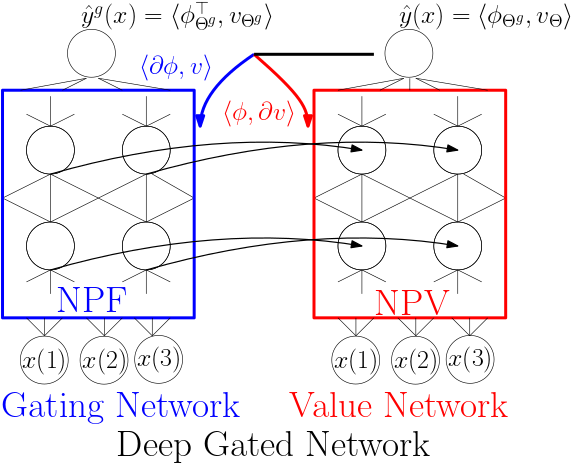
\includegraphics[scale=0.5]{figs/nntwin-blck.png}
}
\end{minipage}
\caption{}
\label{tb:dgn}
\end{table}


%$\begin{aligned}&\text{Learning}\\ &\text{Regime} \end{aligned}$ 